% PS192 Handbook
% Author: Hilduara Abreu
%%%%%%%%%%%%%%%%%%%%%%%%%%%%%%%%%%%%%%%%%%%%%%%%%%%%%%%%%%%%%%%%%%%%%%%%%%%%%%%%%%%%%%%%%%%
\documentclass[11pt, letterpaper]{article}
\usepackage[margin=1in]{geometry}
\usepackage{fancyhdr}
\usepackage{fancyheadings}
\usepackage{titlepic}
\usepackage{pdfpages}
\usepackage[T1]{fontenc}
\usepackage{helvet}
\usepackage{fontawesome}
\usepackage[colorlinks=true, urlcolor=blue, linkcolor=blue]{hyperref}
\usepackage{graphicx}
\usepackage[mmddyyyy]{datetime}
\usepackage{fancyhdr}
\setlength{\parskip}{2mm}
\setlength{\parindent}{0mm}
\setcounter{secnumdepth}{3}
\setcounter{tocdepth}{3}
\usepackage{setspace}
\usepackage{wrapfig}
\hypersetup{breaklinks=true}
\usepackage{verbatim}
\usepackage{fvextra}
\usepackage{float}
\usepackage{lipsum}

% Cover Page
%%%%%%%%%%%%%%%%%%%%%%%%%%%%%%%%%%%%%%%%%%%%%%%%%%%%%%%%%%%%%%%%%%%%%%%%%%%%%%%%%%%%%%%%%%%%%%%%%%
\begin{document}
\sloppy
\thispagestyle{empty}

\includepdf[pages=1,fitpaper]{handbook_front.pdf}

% Header and Footer
%%%%%%%%%%%%%%%%%%%%%%%%%%%%%%%%%%%%%%%%%%%%%%%%%%%%%%%%%%%%%%%%%%%%%%%%%%%%%%%%%%%%%%%%%%%%%%%%%
\pagenumbering{\fancyhf{}}
\pagestyle{headings}
\pagenumbering{arabic}
\fancyhead[L]{\textit{\rightmark}}
\fancyhead[R]{\thepage}
\fancyfoot[C]{The School of Joyful Learning!}
\pagestyle{fancy}
\renewcommand{\footrulewidth}{1px}


% Table of Content
%%%%%%%%%%%%%%%%%%%%%%%%%%%%%%%%%%%%%%%%%%%%%%%%%%%%%%%%%%%%%%%%%%%%%%%%%%%%%%%%%%%%%%%%%%%%%%%%%%

\newpage
\tableofcontents
%\thispagestyle{empty}

% Message from the Principal
%%%%%%%%%%%%%%%%%%%%%%%%%%%%%%%%%%%%%%%%%%%%%%%%%%%%%%%%%%%%%%%%%%%%%%%%%%%%%%%%%%%%%%%%%%%%%%%%%%
\newpage
\section{Message From Principal Abreu}

Dear Staff:

Welcome to the 2023-2024 edition of the PS 192: Jacob H. Schiff  Faculty and Staff Handbook. It is the responsibility of each staff member to be fully acquainted with the information contained herein. This handbook is a living document and it will be updated, as necessary, throughout the year. It is meant to provide information and procedures that are important for the smooth operation of our PS 360 community. This handbook is a guide for ALL STAFF MEMBERS about the daily operation of our school. Please familiarize yourselves with your individual and school-wide responsibilities. Please do not hesitate to ask questions or get further clarification regarding any policy or procedure.

I encourage you to begin by thoroughly acquainting or re-acquainting yourself with our school’s philosophy, mission, objectives and core principles, as outlined in the School Overview. Key elements of this vision are elaborated upon throughout the handbook, along with important information about structures and policies that support our school mission and ensure the safety and success of all members of our school community. 

During the upcoming school year, we will continue to strengthen and deepen our work in relation to NYCDOE and District 6 priorities, as reflected in our School Problem of Practice, priorities and CEP Goals. These areas will be central to our work as a Professional Learning Community and will be further addressed in Professional Learning sessions and Professional Planning Teams, as well as in administrative memos and guidelines, many of which can be accessed in Appendix B of this handbook.

I look forward to our continued collaboration in the year ahead.

Respectfully yours,


\includegraphics[width=0.2\textwidth]{hil_signature}

Hilduara Abreu

Principal

\textbf{The School of Joyful Learning!}

\href{https:www.ps192.org}{www.ps192.org}
\pagebreak
\section{Acknowledgment of Receipt and Review}
Date: \href{https://www.ps192.org}{September, 2023} 

\textbf{Subject: Faculty and Staff Handbook Acknowledgment of Receipt and Review}
\vspace*{0.5in}

I,:\line(1,0){150}(staff member name), hereby acknowledge that I have read and understand the contents of the  Faculty and Staff Handbook, including Appendix A: Chancellor’s Regulations, as well as the PS 192  Family Handbook and Citywide Behavioral Expectations to Support Student Learning.  I understand that I am also responsible for following the directives included in Appendix B: Administrative Memos, as well as subsequent administrative directives that may be issued during the year. I will adhere to the policies and procedures set forth in the PS 192 Faculty and Staff  Handbooks, the Chancellor’s Regulations and in all Administrative Memos.

\vspace{3mm}

\faSquareO \hspace{1em} I have reviewed the The P.S. 192 Staff Handbook

\vspace{10mm}

\begin{center}
\noindent\begin{tabular}{ll}
\makebox[2.5in]{\hrulefill} & \makebox[2.5in]{\hrulefill}\\
Teacher's Signature & Date\\[8ex]% adds space between the two sets of signatures
\makebox[2.5in]{\hrulefill} & \makebox[2.5in]{\hrulefill}\\
Assistant Principal & Date\\[8ex]% adds space between the two sets of signatures
\end{tabular}
\end{center}
\begin{figure}
\begin{center}

\includegraphics[width=50mm,scale=0.5]{himher1}
  \label{fig:school logo}
\end{center}
\end{figure}

\newpage

\section{School Overview} 
PS 192 Jacob H. Schiff (06M192) is a District 6 public school that serves children from diverse cultural, linguistic and socio-economic backgrounds. The success of our students and community relies on our continuous elementary learning experience, dedication, knowledge, teamwork and collaboration. Our school provides a well-balanced looping education that will be a bridge to opportunity and success.To meet our students’ needs, our programs this year will focus on a standards based rigorous curriculum that motivates and inspires students to make connections between our school and their future. We focus on students’ strengths and build self-esteem through authentic and rigorous achievement. We recognize that students can and will value their educational experience because they see, feel and understand the connection to their personal lives.  Preparing our students for College and Career Readiness continues to be at the foundation of all our work.

\begin{wrapfigure}{R}{0.4\textwidth}
\centering
\includegraphics[width=0.6\textwidth]{logohim.jpg}
\end{wrapfigure}

\subsection{Core Values}
At P.S. 192, we uphold a set of core values that serve as the foundation of our educational community. These values, rooted in justice, honor, and self-discipline principles, guide our actions, decisions, and interactions, creating a culture of integrity and excellence.
\begin{itemize}
\item Justice: We are committed to fairness and equality for all members of our school community. We believe in the equitable treatment of every 
individual, irrespective of their background, ensuring that each student has the opportunity to thrive academically and personally. Our commitment to 
justice fosters an inclusive and supportive environment where every voice is heard, valued, and respected.
\item Honor: Integrity is the cornerstone of our educational philosophy. We encourage our students to act with honesty and integrity in all aspects of their lives. Upholding honor means taking responsibility for one's actions, demonstrating ethical behavior, and consistently adhering to a code of moral values. We believe that integrity is the pathway to personal growth and societal betterment.
\item Self-Discipline: We recognize the importance of self-control and self-mastery in achieving success. At P.S. 192, we instill in our students the value of self-discipline as an essential skill for achieving their goals and aspirations. Through self-discipline, our students learn to set priorities, manage their time effectively, and overcome challenges, ultimately becoming responsible and accountable individuals.
\end{itemize}
These core values of justice, honor, and self-discipline guide us in pursuing academic excellence and character development. By embracing these principles, we empower our students to become responsible citizens, compassionate leaders, and lifelong learners who contribute positively to our global community. At P.S. 192, we are dedicated to nurturing academic achievements and the values and qualities that will shape our students into ethical, compassionate, and successful individuals.

\subsection{Vision}
To ensure all students acquire the essential knowledge and skills they need to become independent thinkers, active participants, and contributors in their roles as students and as members of society.

\subsection{Mission}
To provide a welcoming, safe, resourceful, and nurturing environment that supports our school community's academic and social-emotional development where children are respected and engaged in challenging curricula that motivate them to realize their potential as active, lifelong learners. Through our guiding core values of Justice, Honor, and Self-discipline, we aspire to promote perseverance, love, empathy, and respect for oneself and others.

\subsection{School Motto}
"Good, better, best. Never let it rest until your good is better, and your better is best."  -St. Jerome

\section{Educational Philosophy}
We believe that relationships, with oneself and with others, form the basis of learning and teaching. These relationships extend beyond the classroom to include children’s families and the multiple communities of which they are a part. By building meaningful relationships among school, home and the wider community, we seek to instill in each child an integral sense of continuity and connection that will support his or her growth in its many dimensions.

Learning is a natural human process inherent to all children, transcending cultural, socio-economic and learning differences. Children’s innate interests and capabilities are essential to the learning process. A stimulating and engaging environment can awaken a sense of wonder and intellectual curiosity that must be carefully guided and fed. Students learn best when teachers draw upon their existing understandings and help them build new understandings based on increasingly complex knowledge. To this end, our school integrates child-centered pedagogies with rigorous, content-rich instruction in response to ongoing assessment of individual student needs.

\subsection{Core Principles}
The vision for Jacob H. Schiff is guided by the following core principles:
\begin{itemize}
\item An effective learning environment places meaningful relationships—among teachers, students, families and other community members—at its center. 
\item Small learning communities, in which adults and children know each other well, provide rich opportunities for personal, social and intellectual development.
\item Families play an essential role in their children’s education and should therefore be invited to participate in multiple aspects of school life.
\item A community-based school must be accessible, accountable and responsive to all families, regardless of their linguistic, cultural, socioeconomic or educational backgrounds.
\item Children benefit from a coherent academic program that encompasses Pre-Kindergarten to Grade 5.
\item All children have gifts and talents, which can be effectively fostered in heterogeneous classrooms in which adults hold high expectations for every student.
\item Children learn through active engagement and exploration, and by constructing understandings based on their own experiences and observations.
\item A language-rich environment, accessible to children of diverse backgrounds, provides the foundation for achievement in all academic disciplines and areas of life.
\item A well-rounded education provides academic rigor as well as opportunities for self-expression, artistic creation and personal reflection.
\item Engagement in multicultural, multilingual learning environments will prepare children to participate fully in our diverse society.
Education should include not only the mastery of information and skills, but also the development of critical thinking abilities and ethical awareness.
\end{itemize}


\includegraphics[width=1\textwidth]{positivity.pdf}

\subsection{Commitment to Achievement}
In our commitment to delivering a rigorous, inclusive, and family-centered educational experience for the children of our community, PS 192 will:
\begin{itemize}
\item Uphold our identity as a dedicated learning community, earnestly striving to intimately understand each student and their family.
\item Cultivate an intellectually stimulating and captivating learning environment that prioritizes relationships as the primary conduit of both learning and teaching.
\item Assure that our students consistently attain and surpass academic benchmarks across all subject areas.
\item Incorporate family involvement and feedback at various levels of school administration.
\item Instill in every student elevated expectations for their own capabilities, reinforced by unwavering belief in their demonstrated aptitudes.
\item Conduct methodical evaluations of student learning assessments with the aim of scrutinizing data for patterns of misunderstandings and devising solutions to enhance student achievement.
\end{itemize}

\subsection{Commitment to Parental Engagement}
\begin{wrapfigure}{L}{0.4\textwidth}

\includegraphics[width=0.5\textwidth]{logoher.jpg}
\end{wrapfigure}

Research consistently confirms that meaningful family engagement plays a pivotal role in the academic success of children. In light of this, Jacob H. Schiff holds family engagement and authentic home-school partnerships at the core of its mission.

At Jacob H. Schiff, we actively promote meaningful family engagement through regular opportunities for family involvement in classroom activities and school events. Our program design ensures that such involvement aligns with both the school's mission and the educational objectives set by our teachers and staff. Parents and other family members are encouraged to provide various forms of support, which may include preparing classroom materials, delivering curriculum-related presentations about their family experiences or cultural backgrounds, or sharing their expertise in areas such as music, dance, storytelling, science, or technology. Through these collaborative efforts, teachers and family members can establish mutual respect as valued partners in the education of all PS 192 students.

The relationship between the school and families is central to our mission. Consequently, we aspire to foster an active partnership that leverages the unique resources each student brings from their home environment. When families are deeply engaged in their children's learning and children witness their parents' dedication to their education, a vital connection is forged between the home and the school. By cultivating a cooperative partnership with each student's family, our goal is to emphasize the role of families as the ultimate stakeholders in the school and acknowledge their responsibility in the comprehensive education of each child.

As part of our commitment to transparent communication, each grade group is expected to send newsletters to families via grade-level Google groups at least twice a month. These newsletters will provide updates on curriculum developments within the classroom, upcoming field trips, suggestions for family outings and recommended books to enhance your understanding of your child's educational journey within our school.

We look forward to nurturing this strong partnership with you and working collaboratively to ensure the success and well-rounded development of all our students.
\begin{figure}[H]
  \centering
  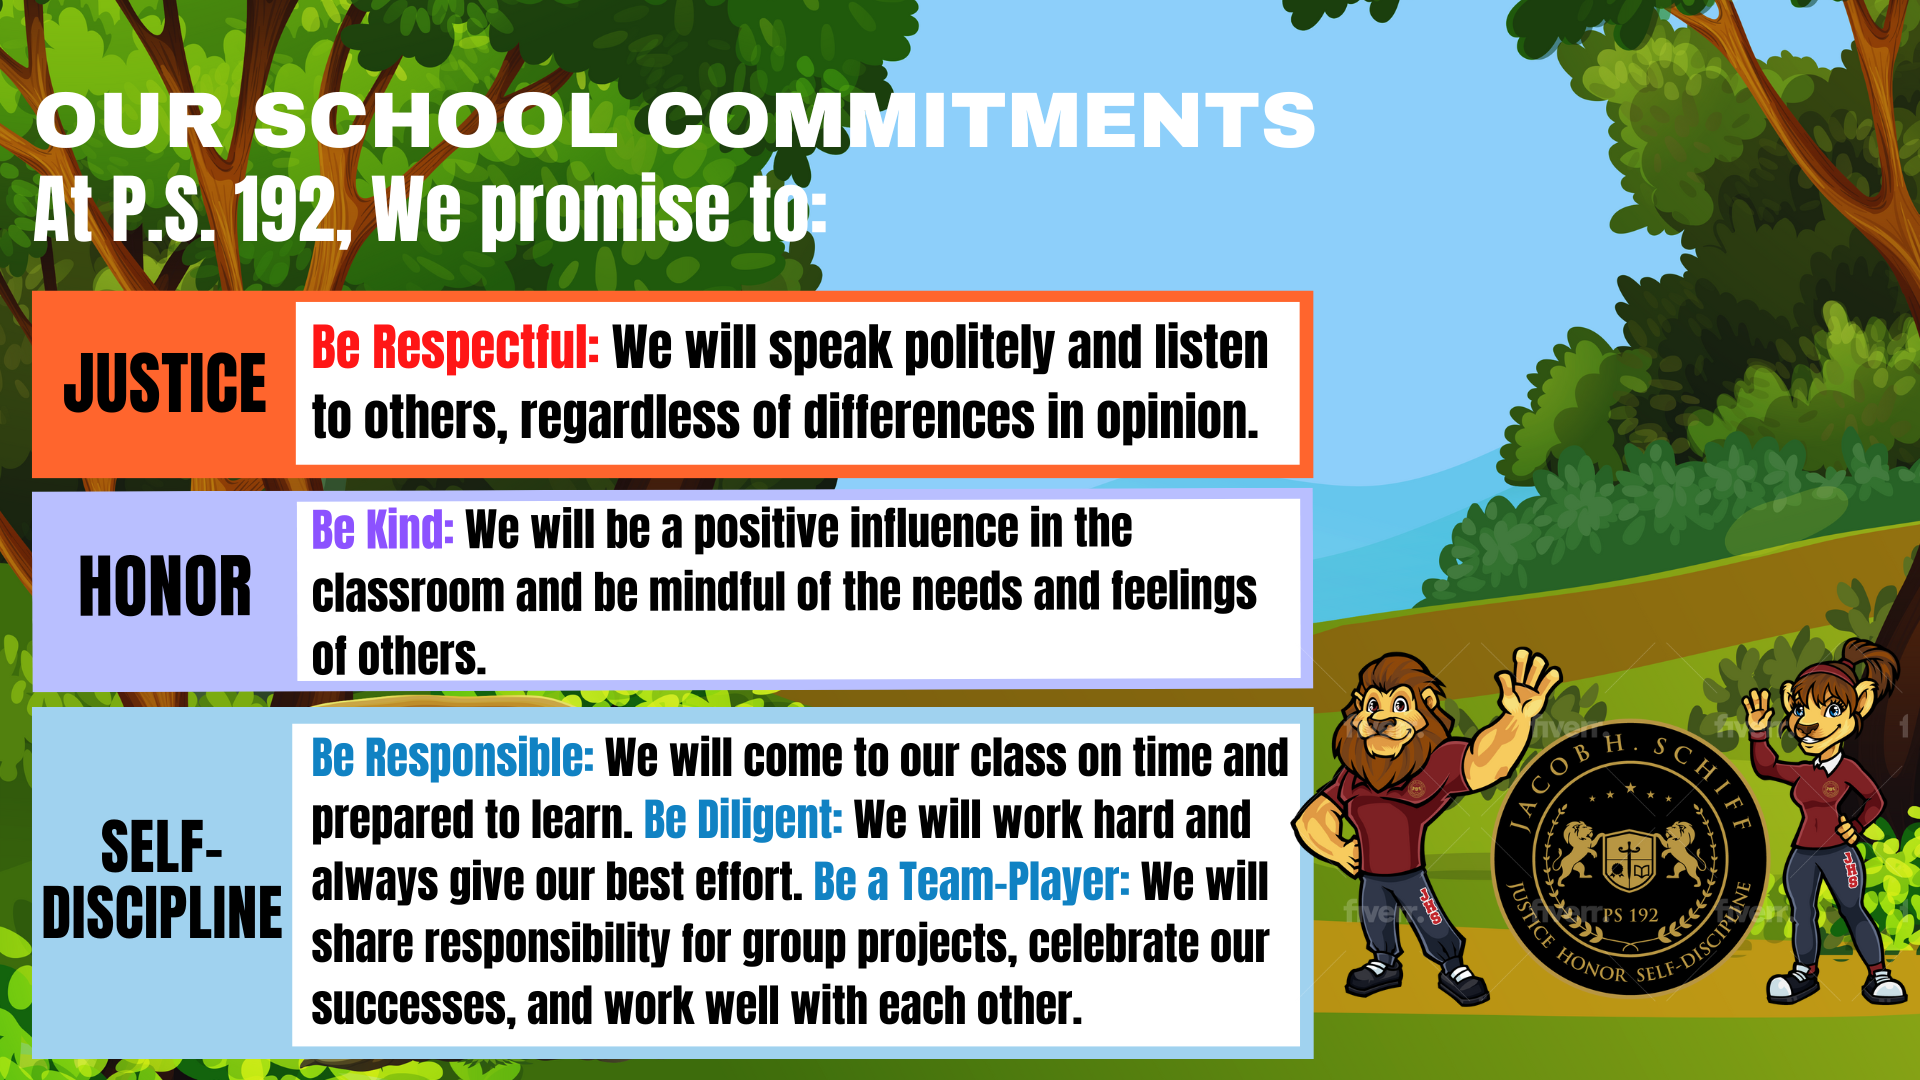
\includegraphics[width=0.9\textwidth]{commitments1}
  \caption{Students Commitments}
  \label{fig:Growth}
\end{figure}
\subsection{Commitment to Community Engagement}
Distinguished educational institutions not only serve as sources of inspiration for students but also maintain intrinsic connections with the communities in which they are situated. A comprehensive and diverse educational program is enriched through hands-on learning, both within and beyond the confines of the classroom. Through the establishment of cooperative alliances with community organizations, our objective is to enhance the Academy's academic curriculum with genuine learning opportunities, extracurricular activities, and avenues for community engagement. Consequently, students can establish profound links between the school and the broader community, fostering their personal, social, and ethical growth, in addition to supporting their academic achievements. This communication aims to inform parents of our commitment to this holistic approach to education.

\subsection{Promoting Positive Student Behavior}
School culture and climate have a profound impact on students’ academic progress and their relationships with peers and adults. Each teacher is expected to promote a positive school culture that provides students with a supportive environment in which to grow both socially and academically. Teachers are expected to take a proactive role in nurturing students’ pro-social behavior. Social emotional learning must is one of the component of a school’s program of universal prevention for all students. 

Effective social emotional learning helps students develop fundamental life skills, including:
\begin{itemize}
\item Recognizing and managing emotions
\item Developing caring and concern for others
\item Establishing positive relationships
\item Making responsible decisions
\item Handling challenging situations constructively and ethically
\end{itemize}
When students develop these skills, they experience more positive relationships with peers, engage in more productive social behaviors, and are less likely to engage in misconduct.

\begin{figure}[H]
  \centering
  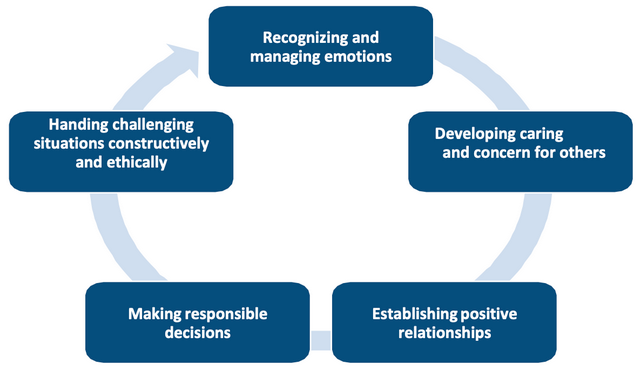
\includegraphics[width=.8\linewidth]{culture.png}
  \caption{\textbf{Our school-wide multi-tiered system of supports (MTSS) is essential to ensuring that the right supports are in place and that we are implementing progressive des-escalation and discipline.}}
  \label{fig:school culture}
\end{figure}

School-wide Positive Behavioral Interventions and Supports (PBIS) is our systems approach to establishing the social culture and behavioral supports needed for all children in a school to achieve both social and academic success. PBIS is an approach that defines core elements that can be achieved through a variety of strategies.

Our Code of conduct is our school-wide behavioral expectation that will support teaching and learning. Students should be able to say what they are and give examples of what they look in action with at least 90\% accuracy.

\subsection{Social, Emotional and Ethical Education}
Research findings support Jacob H. Schiff's emphasis on fostering \href{https://online.harmonysel.org/}{social}, \href{https://online.harmonysel.org/}{emotional}, and \href{https://casel.s3.us-east-2.amazonaws.com/CASEL-Wheel-SEL-Reflection.pdf}{CASEL} \href{https://casel.s3.us-east-2.amazonaws.com/CASEL-Wheel-SEL-Reflection.pdf}{ethical competencies} as substantial contributors to academic achievement. When these educational processes are integrated with academic instruction, students gain the essential tools necessary for a lifelong commitment to learning and responsible citizenship. Therefore, it is imperative that WHA teachers actively incorporate these skills throughout all facets of the curriculum. Collaboration between teachers, school staff, and family members is essential to collectively develop and exemplify the adult competencies we aspire for our children to emulate.

\begin{figure}[H]
  \centering

\includegraphics[width=1\linewidth]{1.png}
\caption{\textbf{The School of Joyful Learning!}}
  \label{fig:PS192}
\end{figure}

\subsection{The Pre-Kindergarten–Grade 5 Looping Model}
Jacob H. Schiff has been implementing since 2021, offers students a continuous elementary learning experience—a model that holds value for many families and aligns with educational research. Looping, as defined by Cistone et al. (2004) in Hill (2018, p. 2), is "a policy in which whole classes (or most of the students within a class) are taught by the same teacher in sequential years." This practice, also known as "continuous learning," has demonstrated both quantitative and qualitative benefits within a school setting. A recent seminal study shows that looping can lead to improved test scores, with the most significant effects observed among minority students (Hill 2018, p. 2, Franz et al. 2010, Cistone et al. 2004, Bogart, V. 2002). Furthermore, it positively impacts student attendance and their progression to the next grade (Cistone, et al. 2004).

Daggett's Effectiveness and Efficiency Framework highlights classroom looping as one of the practices worth considering, ranking it second on the list (Beilefeld 2016). Daggett presents looping as a "low-cost, high-effect" approach for modern schools, a sentiment echoed by Hitz (2007), who emphasizes that looping is not a complex undertaking. Looping contributes to a positive school culture by reducing transitions and increasing trust in relationships with students and parents (Rassmussen 1998, Chaika 2009).

Schools that have effectively implemented the looping structure have reported several benefits, including improved relationships among students and between teachers and students, more efficient instruction, improved attendance rates (5\%), reduced student grade level retention (43\%), fewer referrals of students to special education programs (55\%), and improved student discipline (Grant 2017). Staff attendance also improved, with an average reduction from 7 days absent to just 3 days absent (Grant 2017).
\section{School Day Procedures}
The instructor assumes responsibility for each student within their assigned class throughout the entirety of the school day, regardless of their location within the school premises. It is imperative that a certified adult presence is maintained in the classroom for as long as a single student is present.

Students are not permitted to move within the school building without the supervision of either an instructor or a paraprofessional. This rule applies to transitions to and from specialized rooms (such as the art studio, library, auditorium, and gym), as well as movements during lunch/recess and during morning arrival and end-of-day dismissal procedures. Stairwell B has been designated for use by PS 192 for travel to and from classrooms.

The only exception to this rule is applicable to students in grades 2 through 5 who may be allowed to visit the main office unaccompanied, solely for the purposes of delivering the attendance folder or seeking early dismissal.

\subsection{Lesson Plans}
As we forge ahead in our collective quest to deliver top-tier instruction to our students, it's imperative that we work together efficiently and effectively. With this in mind, I'd like once again to highlight the critical role of lesson planning and the importance of having your daily plans for each subject printed and ready before your workday begins.

Preparing your lessons beforehand not only maximizes our teaching time but also fosters a more dynamic, data-informed, and focused social-emotional and educational atmosphere for all learners. It sets the stage for us to define explicit objectives and arrange our teaching/behavior strategies and discussion framework. By planning your lessons in advance, you not only optimize instructional time but also bring joy to everyone.

Every staff member has been granted access to a printer, printing paper, ink, and a lesson plan binder to facilitate an effortless process of keeping your lesson plans accessible and organized when requested by an administrator. Teachers, cluster teachers, and service providers are required to print the daily plans by no later than 8:00 a.m.- the commencement of our school day- to further contribute to a smoother operation within the classroom and reduce disruptions during instructional time to 0%.

Moreover, classroom teachers must provide guidance and assign the instructional tasks that will be carried out by teacher assistants. This will provide them with the opportunity to familiarize themselves with and prepare any materials required to effectively carry out the tasks outlined in the teacher's lesson plan. Teacher assistants are obliged to keep a daily log detailing the activities they have conducted and the students they have assisted.

Your daily Lesson plan must include the following elements:
\begin{itemize}

\begin{figure}[H]
  \centering
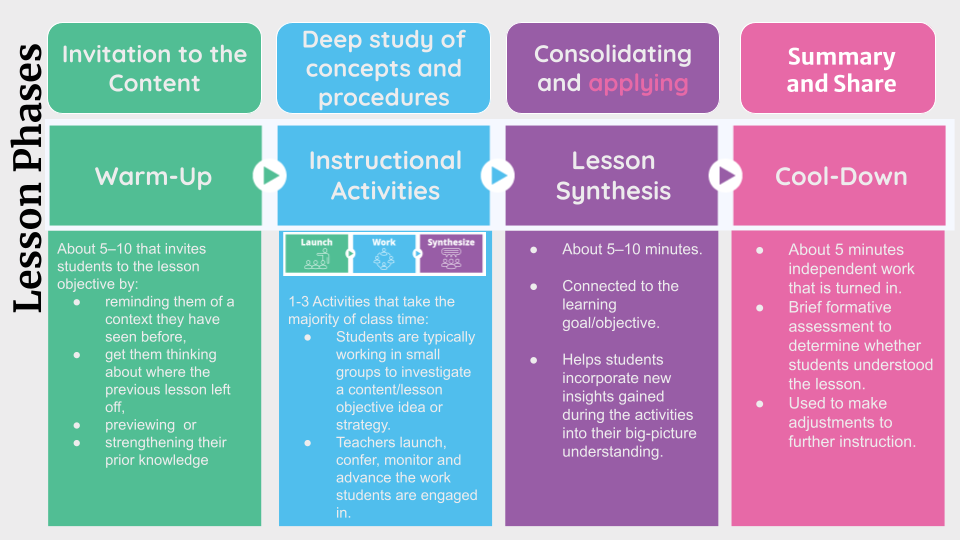
\includegraphics[width=1\linewidth]{lesson_instructional_phases.png}
\caption{\textbf{Lesson Phases Chart}}
  \label{fig:lesson-phases}
\end{figure}

\item \textbf{Objetive(s)}: Clearly define the learning objectives, target, or goals of the lesson. What should students know or be able to do by the end of the lesson? “I can...”
\item \textbf{Standars}: Reference the relevant academic standards that align with the lesson.
\item \textbf{Duration}: Indicate the estimated time needed to complete each section of the lesson.
\item \textbf{Materials and Resources}: List all materials, resources, and technology required for the lesson, including textbooks, workbooks, multimedia, or any other tools.
\item \textbf{Pre-assessment}: Describe how you will assess students' prior knowledge or skills related to the lesson topic.
\item \textbf{Integration}: If relevant, indicate how the lesson integrates with other subjects or disciplines.
\item \textbf{Safety Considerations}: Include any safety precautions or considerations if they apply to the lesson.
\item \textbf{Introduction}: Explain how you will engage students and introduce the lesson's main concept or topic.
\item \textbf{Instructional Strategies}: Outline the teaching methods, strategies, and activities you will use to convey the lesson content. Be sure to include differentiated approaches to meet the needs of diverse learners.
\item \textbf{Grouping and Differentiation}: name and specify how students will be grouped, whether by ability, interest, or other criteria. Describe how you will differentiate instruction to meet the needs of various learners, including those who may need additional support or challenges. (Guided literacy, guided math, and guided writing plans)
\begin{itemize}
\item \textbf{Accommodations and Modifications}: Detail any accommodations or modifications for students with special needs or diverse learning styles.
\item \textbf{Language Support}: Describe how you will support English language learners (ELLs) or students who require language assistance.
\item \textbf{Engagement and Discussion Strategies}: Highlight strategies and discussion protocols to keep students cognitively engaged and motivated throughout the lesson.
\end{itemize}
\item \textbf{Assessment and Formative Assessment}: specifically name and describe the methods you will use to assess students' understanding during the lesson. Include both formative assessments (ongoing checks for understanding) and a summative assessment to evaluate the lesson's overall success.
\item \textbf{Closure}: Explain how you will wrap up the lesson, summarize key points, and connect the content to the learning objectives.
\item \textbf{Homework or Follow-Up}: specify any homework assignments or follow-up activities that students should complete outside of class.
\item \textbf{Cluster Teachers}: Specify the class for which the lesson is designed. For example, Class 201. Each lesson plan must be tailored to the needs of each individual class
\item \textbf{Optional: Best practice Tip}: Reflection: Provide space for reflection on the effectiveness of the lesson and any adjustments you might make when teaching it again
\end{itemize}
 Let's remember our shared dedication to providing an excellent education for PS 192 students. By prioritizing lesson planning and printing daily plans, we are not only making our jobs easier but also contributing to the overall social emotional, and academic growth and success of our students.

If you have any questions or need any of the resources listed in this email, please don't hesitate to reach out to Ms. Macdonald, Ms. Rodriguez, or me. We are here to support you and work as a team to achieve our goals.

Together, we can create an exceptional learning experience for all of our students.

\subsection{Arrival} 
Breakfast is served within the cafeteria from 7:40 to 7:55 am. If a student intends to partake in breakfast at school, they should enter the cafeteria during the designated time frame of 7:40 to 7:55 am. School staff will ensure that students who choose to have breakfast at school are escorted to their respective classrooms by 7:59 am.

All students in grades K-5 are required to assemble in the yard during arrival. Parents are kindly requested not to accompany their child into the school building. However, on the first day of school, Kindergarten and transfer students may be accompanied by a parent/guardian into the school.

Please be mindful of our shared facility with PS 229 during both Arrival and Dismissal. To maintain a smooth flow, we should refrain from entering the school front door during the arrival or dismissal times of PS 229, which occur 10 to 20 minutes before our own. PS 192 families are kindly asked to wait until a PS 192 staff member opens the gate before entering.
\subsection{Student Attendance}
Children cannot attain their full potential, both academically and socially, if their attendance exhibits irregularity. The absence of consistent participation in instruction and the disruption of their ability to form connections with peers and curriculum significantly jeopardizes a child's developmental progress.

Students arriving late find themselves endeavoring to catch up with the classroom's tone and pace. Therefore, we strongly urge parents to accord utmost importance to both attendance and punctuality.

Our school policy stipulates that students should be present in school every day from 8:00 AM to 2:20 PM. There is a brief grace period of 5 minutes, and no student should be marked as late until after 8:05 AM. In cases of late arrivals, Shalymet Cuesta maintains records in our attendance notebook, which serves as a supplementary record. If a child has been initially marked as absent, kindly ensure that the attendance sheet is amended to reflect lateness. If the attendance folder has already been submitted, any recorded absence will be duly adjusted to reflect lateness by Shalymet Cuesta in the main office.

Each class is equipped with an attendance folder that contains the scan sheet and a comprehensive list of students. Teachers bear the responsibility of meticulously recording student attendance.
\begin{figure}[h]
  \centering

\includegraphics[width=1\linewidth]{2.png}
\caption{\textbf{The Lion's Den}}
  \label{fig:school mascots}
\end{figure}
In the event of concerns regarding a student's attendance, teachers should initially engage in direct communication with the parent(s)/guardian(s). Should the issue persist, teachers are encouraged to escalate it to Rijo, Cuesta, or Estrella. If the problem remains unresolved, please contact Javier.

Please take note that excessive absences and/or tardiness may be construed as educational neglect, warranting reporting to the New York State Agency for Child Services (ACS).

Upon completion of attendance, it is imperative to dispatch the attendance folder to the school office by 9:15 AM. 
\begin{itemize}
\item The folder will be made available in each teacher's mailbox prior to 8:00 AM. In the event that it is not found in your mailbox by 8:00 AM, it will be delivered directly to your classroom. 
\item Attendance must be recorded promptly upon the class's entry into the room, and attendance forms must be diligently completed on a daily basis, serving as a vital backup for our records. 
\item To ensure that attendance data is entered into the Attendance Tracking System (ATS) before the daily deadline, the attendance folder must be returned to the school office no later than 9:15 AM, with the classroom teacher(s) ultimately responsible for verifying its accuracy.
\end{itemize}
\begin{Verbatim}[breaklines=true, breakanywhere=true]
It is of paramount importance that attendance is meticulously documented, as these records constitute official and legal documents of the highest significance.
\end{Verbatim}

\section{Crisis Intervention Plan}
\begin{itemize}
\item Crisis Intervention First Responders: 
	\begin{itemize}
	\item Point Person for Grades K-2: Ms. Lynette Hernandez X1282
	\item Point Person for Grades 3-5: Ms. Luisa Estrella X2262
	\end{itemize}
\end{itemize}
\subsection{What is Tier 1 Support?}
Tier 1 systems, data, and practices support everyone across all settings. They establish the foundation for delivering regular, proactive support and preventing unwanted behaviors. Tier 1 emphasizes modeling, teaching, and acknowledging positive social, emotional, and behavioral (SEB) skills. 

The core principles guiding Tier 1 include the understanding that we can and should:
\begin{itemize}
\item Effectively teach appropriate SEB skills to all students.
\item Differentiate instruction for behavior
\item Intervene early before unwanted behaviors escalate
\item Use research-based, scientifically validated interventions whenever possible 
\item Clearly define consequences for unwanted behaviors
\item Monitor student progress
\item Use data to make decisions
\end{itemize}
\subsubsection{Tier I De-Escalation Strategies}
\begin{itemize}
\item Act calm
\item Give a choice:— a simple, quick, calm, respectful way of letting a student know about the unwanted behavior and what they could do instead. \href{https://www.instagram.com/reel/CfmyGhJgWzb/?utm_source=ig_embed&ig_rid=a26d419e-f673-4b9f-8a6a-0d678307a527}{Video on the choice strategy}
\item Change the subject to a positive one: \href{https://www.instagram.com/reel/CUWGczxARq_/?utm_source=ig_embed&ig_rid=fd9f8bf6-5411-4874-9486-3ba446bc2fc0}{Redirect behavior}
\item \href{https://www.pbisapps.org/articles/slow-the-climb-4-de-escalation-strategies-to-keep-behavior-from-going-downhill}{Remind them of a strategy they know}
\item Co-regulate when they can self-regulate
\item Invite students to to a calming activity (breathing, drawing, journaling)
\item Co-regulate when they can self-regulate
\item Invite students to to a calming activity (breathing, drawing, journaling)
\item Give space and wait time
\item Use a behavior progress report (must be signed by parent on a daily or weekly basis)
\item 1-1 conference with student and/or guardian
\end{itemize}
\subsection{What is Tier 2 Support?}
\begin{itemize}
\item Crisis Intervention First Responders: 
\begin{itemize}
\item Point Person for Grades K-2: Ms. Lynette Hernandez X128
\item Point Person for Grades 3-5: Ms. Luisa Estrella X226
\end{itemize}
\end{itemize}
The core principles guiding Tier 2 include the understanding that we can and should:
\begin{itemize}
\item Progress monitoring for at risk students 
\item Create structures and predictability:  Intervene early before unwanted behaviors escalate by anticipating triggers and possible solutions 
\item Weekly meeting with the Crisis Intervention team for increasing contingent adult feedback 
\item Analyze academic and behavioral performance
\item Increase home/school communication 
\item Collect and use of data for decision-making 
\item Basic-level function-based support
\end{itemize}
\subsubsection{Tier II De-Escalation Strategies}
\begin{itemize}
\item Act calm
\item Be empathetic and nonjudgmental. ...
\item Avoid overreacting. ...
\item Set positive limits. ...
\item Ignore challenging questions. ...
\item Allow quiet time for reflection. ...
\item Do a quick body scan. ...
\item Use diffusers to de-escalate. ...
\item Practice reflective teaching ...
\item 1-1 conference with students and/or guardian
\item Small group counseling sessions
\end{itemize}
\subsection{Tier 3}
\begin{itemize}
\item Crisis Intervention Team:
\end{itemize}

\section{Professional Expectations}
\subsection{Teacher Criteria:}
At Jacob H. Schiff, a foundational tenet of our educational philosophy revolves around a team-based approach to teaching and learning. In alignment with our school's overarching mission, our dedicated educators engage in collaborative efforts to meticulously design curriculum and instructional strategies. They employ a diverse array of assessment tools to thoughtfully analyze student progress, thereby informing and enhancing our teaching methods.

This collaborative planning plays a pivotal role in ensuring the seamless alignment of curriculum objectives and fostering instructional uniformity across various classrooms and grade levels. Furthermore, our teachers operate within collaborative teams to actively support the holistic growth of our students, encompassing their social, emotional, and ethical development. This comprehensive approach underscores our commitment to providing a well-rounded education for your child.

\begin{figure}[H]
  \centering

\includegraphics[width=1\linewidth]{4.png}
\caption{\textbf{"Today and every day, let justice guide your actions, honor inspire your choices, and self-discipline be the key to unlocking your potential. You are the future of a brighter, fairer world."}}
  \label{fig:school symbol}
\end{figure}

All personnel are expected to embrace and promote the mission, philosophy, and fundamental tenets of PS 192: Jacob H. Schiff, and must either possess or be open to acquiring the following skills and attitudes:
\begin{itemize}
\item Operate effectively within a highly collaborative environment, necessitating active, suitable, and proficient communication with peers, parents, students, and other stakeholders.
\item Adapt to the school's timetable and organizational structure, tailored to meet the diverse backgrounds and requirements of our students.
\item Engage in interdisciplinary planning and teaching teams with a primary focus on integrating social and emotional learning into every facet of instruction.
\item Adopt an open-door policy to foster the development of best-practice pedagogy and facilitate professional growth through collaboration.
\item Utilize a variety of assessment methods and student data to guide effective instruction.
\item Review, apply, and ensure the provision of services, modifications, and accommodations as outlined in IEPs (Individualized Education Plans) for SWD (Students with Disabilities) in compliance with their entitlements.
\item Effectively manage classrooms populated with diverse learners, utilizing flexible and cooperative groupings, as well as targeted whole-class instruction to address varying learning styles, academic proficiency levels, and social-emotional needs.
\item Incorporate project-based work and instruction across various content areas.
\item Devise and execute challenging, engaging units that encourage critical thinking and culminate in completed student works, 
contributing to a growing portfolio.
\item Seamlessly integrate technology as a teaching tool within the classroom.
\item Create meaningful opportunities for family involvement within the classroom and throughout the school, including workshops and resources.
\item Contribute to and participate in special programs, such as workshops and curriculum nights, with a particular emphasis on engaging families.
\item Engage in after-school and Saturday programs, attend planning sessions, and potentially contribute to summer planning and curriculum development.
\item Report to the assigned post by 8:00 a.m. daily, as any arrival after 8:00 a.m. will be considered tardy.
\item Adhere to the prescribed program schedule, punctuality in all classes, Related Services sessions, and fulfill all assigned duties and responsibilities.
\item Maintain readily accessible daily lesson plans or session plans upon request, utilizing a provided lesson plan binder for organization and accessibility, which should be placed atop the portfolio shelf near the entrance.
\item Regularly check and respond to emails and review the office communication board.
\item Attend to office mailboxes at the start and end of each day.
When departing the building for lunch or meetings, ensure completion of the sign-out book and consult with our secretary, Ms. Dulce Infante, before leaving.
\item Following attendance at professional learning sessions or workshops during work hours, provide proof of attendance and an agenda within 48 hours to Ms. D. Infante, in either hard or soft copy format.
Initiate daily attendance taking at the outset of each day, preserving records and placing the red attendance folder in the exterior compartment adjacent to your classroom door. This requirement applies solely to classroom teachers and substitute teachers.
\item Complete the sign-out book, situated at the classroom entrance, when removing a student from the classroom for the provision of Related Services or evaluation.
\item Maintain close supervision of students at all times. During the school day, students are not permitted to exit the school premises unless signed out at the welcome center by an adult aged 18 or older, whose name must be listed on the emergency contact card. Outside of dismissal hours, teachers may not release a child to anyone not listed on the blue card without administrative approval. The official teacher is responsible for the whereabouts of their assigned students at all times. Should another staff member redirect a student, the homeroom teacher must be informed. Students from different classes should not enter your classroom without prior notification via classroom phone or written communication. In grades 4-5, students may travel within the building independently with a pass, but they must never be left unattended. In the event of leaving the room, students must be entrusted to the care of another adult. In emergencies, contact the main office, a supervisor, or another staff member for assistance. Group movement of students within the building must always include adult accompaniment. Under no circumstances should students be left unattended in hallways or anywhere within the building. Immediate notification to the main office is imperative in the following situations: 
\begin{itemize}
\item if a student departs from your room without permission
\item fails to return from lunch or a bathroom break
\item or goes missing for a duration exceeding 5 minutes, in order to promptly inform parents.
\end{itemize}
\item Keep inform:
\begin{itemize}
\item Regular staff memos and emails are routinely disseminated, conveying important updates, timelines, and newly implemented policies that require your attention. It is imperative that you diligently review these communications and take appropriate action in response. Neglecting to read the memos does not absolve you from the responsibility of being informed about their contents.
\item Please be advised to routinely monitor the White Message Board located within the main office, as well as your Department of Education (DOE) email, for important notifications. Furthermore, we kindly request that you regularly check your DOE email for updates regarding professional development opportunities, per-session postings, meetings, and related matters. Your vigilance in this regard is greatly appreciated.
\end{itemize}
\item Ensuring Parental Communication: It is expected that each grade group will diligently transmit a newsletter to their respective families through the grade-level Google Groups no less than twice per month. This newsletter should comprehensively detail curriculum advancements within the classroom, forthcoming excursions, suggestions for family leisure activities and literature for communal exploration, relevant articles, and any other pertinent information aimed at enriching families' comprehension of their child's experiences within our school environment.
\end{itemize}
\begin{Verbatim}[breaklines=true]
Adequate prior notification and appropriate compensation will be duly afforded. While teacher involvement in these activities is voluntary, we strongly encourage it, as their participation is integral to the school's overall success.
\end{Verbatim}
\section{Professional Conduct}
In accordance with Jacob H. Schiff School's vision and objectives, we kindly request that all members of our staff maintain the utmost professionalism in their conduct at all times. Our school's expectations for professional comportment encompass the following facets: adherence to appropriate school attire, a commitment to honesty, the demonstration of courtesy in interactions with others, the preservation of confidentiality, and the maintenance of suitable professional boundaries when engaging with administrators, colleagues, students, and their families.
\subsection{Unacceptable professional behaviors} 
\begin{itemize}
\item Misconduct: This category encompasses, but is not restricted to, actions such as the falsification of records, engaging in financial dishonesty, committing fraud, engaging in misrepresentation, forgery, or theft.
\item Defiance of Authority: This category encompasses, but is not restricted to, the refusal to comply with directives provided by supervisory personnel.
\item Non-Cooperation: This category encompasses, but is not restricted to, the failure to collaborate with appropriate staff members in the execution of their duties and responsibilities.
\item Subpar Job Performance: This category encompasses, but is not restricted to, an inability or unwillingness to carry out assigned duties and/or to meet the school's established performance standards. It also includes recurrent absenteeism or tardiness.

\begin{figure}[H]
  \centering

\includegraphics[width=1\linewidth]{3.png}
\caption{\textbf{"We are PS192!"}}
  \label{fig:school motto}
\end{figure}

\item Unprofessional Behavior: This category encompasses actions such as failure to maintain appropriate boundaries with students or families, displaying rudeness towards others, or engaging in conduct that demonstrates a lack of respect for fellow members of the school community, including students, staff, and administrators.
\item Actions Contrary to the Best Interests of the School: This category encompasses, but is not restricted to, actions that may be detrimental to the school's overall welfare and objectives.
	\begin{itemize}
	\item In order to maintain a formal and respectful environment within our school community, we wish to communicate the following guidelines and policies:
	\begin{itemize}
	\item Public Commentary and Confidentiality: It is imperative that we refrain from any public disparagement of the school’s staff, students, or families and avoid any breach of confidentiality.
	\item Cellular Phone and Headphone Usage: During instructional time or work hours, the use of cellular phones, headphones (including iPods and earpieces), and similar devices is strictly prohibited for personal use. These devices, including texting, should only be activated during free duty lunch breaks. Please refer to the email sent on 9-7-2023 for more information.
	\item Classroom Telephone Usage: Classroom telephones are to be used exclusively for school-related matters. We kindly request that you inform your family and friends about this policy, emphasizing that classroom phones are solely for communication with the main office and should not be used for classroom-to-classroom calls.
	\item Replying to All for Individual Concerns: Avoid creating confusion or chaos by utilizing the "reply to all" function when addressing individual concerns.
	\item Email Communication: To maintain effective communication, please refrain from emailing the entire staff or sub-groups of staff members without prior approval from the principal.
	\item Laboratory Usage: Excessive use of laboratory facilities during instructional time or work hours, without medical accommodation, is discouraged. In the event of an emergency, please contact Ms. Infante at extension 1240, and a member of the administrative team will assist you.
	\item Visiting During Instruction: We kindly request that staff members refrain from visiting colleagues during instructional sessions to ensure an uninterrupted learning environment.
	\item Utilization of Prep Periods: Please adhere to the utilization of prep periods as outlined in the Teacher’s UFT contract.
	\item Respect During Meetings: Disrupting Marvelous Monday and/or teacher team meetings by playing music on a digital device while the meeting is in session is discouraged and should be avoided.
	\item Music in Hallways: The playing of music on digital devices in the hallway requires prior administrative approval.
	\end{itemize}
\end{itemize}

\begin{Verbatim}[breaklines=true, breakanywhere=true]
By adhering to these policies and guidelines, we can maintain a professional and focused educational atmosphere that benefits both our dedicated staff and the wonderful students we serve. Your cooperation in upholding these standards is greatly appreciated, as it contributes to a positive and productive school environment. Thank you for your understanding and support.
\end{Verbatim}
\item \textbf{Breach of Confidentiality:} This encompasses the utilization of confidential information for personal gain or the unauthorized disclosure of such information without proper authorization or approval.
\item \textbf{Contravention of Department of Education (DOE) Policies on Substance Use and Smoking:} This encompasses, though is not restricted to, the illicit use of controlled substances, consumption of alcohol, and smoking on school premises
\end{itemize}
\section{Health and Wellness}
\subsection{School Nurse}
PS 192 and Ms. 209 jointly employ a full-time school nurse who maintains her office on the first floor of the school premises. In the event that a child sustains an injury while on school grounds, our dedicated nurse is readily accessible to provide assistance.

When necessitating the attention of the school nurse for your child, we kindly request that you complete a requisite form prior to sending your child to the nurse's office. Furthermore, as a safety precaution, we require that all students be accompanied by an adult when escorting them to the nurse's office. For students in grades 3-5 who have been identified as responsible and trustworthy, they may also be accompanied by a designated "buddy" during this process.

Ensuring the well-being of our students is of paramount importance to us, and our school nurse plays a vital role in this regard. Your cooperation and understanding in adhering to these procedures are greatly appreciated as we strive to maintain a safe and nurturing environment for all our students.
\subsection{Administration of Medication:}
In the event that a child necessitates regular medication administration, the school nurse will request the completion of a Medication Administration Form (Form 504), obtainable either online or from the Nurse's office. This document must be duly filled out by the child's attending physician. Unless expressly designated for self-carry and self-administration, all medications, including items such as asthma pumps, aspirin, and allergy medication, will be securely stored within the nurse's office and solely dispensed by the nurse.

While our school nurse strives to maintain updated medical records, we kindly request incoming parents to proactively provide any pertinent updates regarding their child's medical conditions or allergies. We recommend reviewing the information on your blue emergency contact cards and ensuring that any health-related issues are duly noted before submitting these blue cards to the school office.

In situations where a student possesses a life-threatening allergy, the school may equip teachers with and provide training on the use of an epi-pen, which will be readily accessible within the classroom. Your understanding and cooperation in this matter are greatly appreciated.
\subsection{Illness:}
In the event that a child displays symptoms of illness or appears unwell, it is imperative that they be escorted to the Nurse's office located on the first floor. The child may choose to recuperate either in the Nurse's office,\textbf{which also serves as the SAVE room}, or in a dedicated area within the school office designated for such instances. Please ensure that the child is accompanied by a note detailing the reasons for their visit when sending them to the nurse's office.

Should a student's condition deteriorate to the extent that they are unable to make their way to the nurse's office, kindly request the nurse's presence in your classroom and promptly notify a school administrator or a member of the guidance team. It is essential that any situation involving an ailing student be communicated to their parent or guardian. The responsibility for making contact with the parent rests with an adult figure, be it a teacher, student teacher, parent coordinator, office personnel, or an administrator. We kindly request that students refrain from making direct calls to their parents in such instances. If you encounter students who frequently seek to consult the nurse, we encourage you to engage in a discussion with an administrator regarding the matter.

In the unfortunate event of a child sustaining an injury during the school day, including minor incidents resulting from routine school activities, it is imperative that the parent or guardian be promptly informed. If the child has received medical attention from the nurse, a written record of the visit to the medical room will be sent home. In cases where the child has not sought the nurse's assistance, it becomes the responsibility of the teacher or supervising adult present during the incident to convey the information to the parents. Furthermore, \textit{if any visible marks or injuries are observed, we strongly urge the teacher to make every effort to reach out to the parent, whether at their workplace or residence, prior to the conclusion of the school day, in order to provide an update on the child's condition}.
\subsection{Incident Reports:}
Any instances of accidents, incidents, or injuries involving students or staff members must be promptly reported prior to leaving the school premises on the day when such incidents occur. Additionally, it is imperative to submit a written report to our Assistant Principal, Ms. Arelis Javier, before departing the building. Should a school nurse be present on the premises, it is mandatory for the affected student or staff member to seek immediate medical attention from the nurse. The incident report will be documented in the Online Occurrence Reporting System (OORS) within 24 hours of its initial notification.

If a student arrives at school with visible marks, bruises, casts, or any other discernible injuries that were not evident the previous day, it is essential to conduct a private conversation with the student. Should any concerns arise during this conversation, it is imperative to promptly refer the student to the school nurse. Simultaneously, please provide a note detailing your concerns and inform the main office, the administration, and/or the guidance department. In cases where necessary, report the incident to the New York State (NYS) hot-line with the assistance of a member from the guidance team. It is crucial to note that all school staff members are mandated reporters, and it is essential to consult your training materials and yearly refresher handouts for further guidance.
\subsection{Safety and Emergency Preparedness}
These protocols and procedures have been meticulously crafted to ensure the safety and well-being of our students, faculty, and visitors, all while preserving a hospitable and inclusive atmosphere. We deeply value the collective cooperation of all individuals in adhering to the PS 192 Visitor and Safety Guidelines and Procedures. To guarantee the safety of every person within our premises, the following safety measures are currently enforced:
\begin{itemize}
\item A dedicated security guard is consistently stationed at the main entrance of the facility.
\item For students departing before the scheduled end of the school day, it is imperative that they are signed out by an authorized adult in the presence of staff members from the Welcome Center. During regular school hours, only individuals aged 18 years or older are permitted to sign out students. No student sign-outs will be allowed between 2:00 PM and 2:20 PM.
\item All visitors entering the premises are required to furnish a valid photo identification to the on-duty security personnel and subsequently register at the Welcome Center, located in Room 119.
\item Each family is kindly requested to complete an annual emergency form, often referred to as the "Blue Card," which should include the contact information of parent(s)/guardian(s), in addition to a list of three or more trusted friends or family members who can be contacted in case of an emergency. At the outset of the school year, teachers and the school nurse will be provided with the parent/guardian's primary contact number, with any additional contact information accessible through the main office.
\item All individuals, including visitors and staff, are expected to strictly adhere to the PS 192 Visitor and Safety Guidelines and Procedures.
\end{itemize}
\begin{Verbatim}[breaklines=true, breakanywhere=true]
These measures are communicated to inform all school staff members and stakeholders of the protocols that contribute to the safety and security of our school community. Your unwavering commitment to these guidelines is essential in maintaining a secure and nurturing educational environment for all.
\end{Verbatim}

\subsection{Inter-visitations}

\begin{figure}[H]
  \centering

\includegraphics[width=1\linewidth]{5.png}
\caption{\textbf{“Today, we stand tall, celebrating a remarkable ascent to 7th place in ELA and 10th in Math"}}
  \label{fig:school success}
\end{figure}  

\begin{itemize}
    \item In our continuing efforts to build professional capacity and enhance our school-wide effectiveness in improving teaching and learning, professional development for all staff is a major priority.  Classroom inter-visitation is a potentially powerful way for us to share our best work with each other, as we build and nurture  our school’s professional learning community.
    \item In order to ensure that classroom inter-visitation among staff are purposeful, productive, and aligned with our school’s CEP goals and objectives, it is important for me to clarify guidelines for all staff to follow.
    \item These guidelines are:    
    \begin{itemize}
        \item Be certain to submit a written request (official inter-visitation request form) at least 72 hours in advance, to Ms. Abreu
        \item Your request will be reviewed and approved (or not approved) by the supervisor in charge. You must wait for official approval before visiting another teacher’s class.
        \item When visiting a colleague’s class, please refrain from any conversations during instructional time.  All conversations must be conducted during preparation periods or any other mutually convenient times, but NOT during instructional time. 
        \item Be sure to fill out and submit the official school Post inter-visitation form to Mrs. Abreu, within 48 hours after your visit.
        \item It iis expected that teachers who visit other classes to enhance and improve their own teaching practices will be accountable for implementing these best instructional strategies observed  in their own classes.
    \end{itemize}
    \item While I fully endorse and encourage professional collaboration in our school, it is essential that all teachers adhere to the guidelines above and that all staff members ensure that teachers remain focused on their primary and professional responsibility, which is the direct teaching and supervision of the students in the class, during assigned instructional periods.
    \item All other professional development/learning opportunities need Mrs. Abreu's prior approval.
\end{itemize}

\subsection{Safety}
    Please familiarize yourself with these instructions and review them with your students. The school will train and drill all staff and students in the General Response Protocol in September, which describes what to do in an Evacuation, Shelter-In, Hold or Lockdown Drill. It is your professional responsibility to understand the safety guidelines provided. It is strongly recommended that you review, frequently, the  Safety Opening Day Presentation.

For any concerns or inquiries from parents or family members, kindly direct them to Ms. Angela Rijo or Ms. Arelis Javier (Zoom link will be provided).

All other staff members, including guidance personnel, psychologists, social workers, secretaries, and others, are expected to utilize the time for job-related tasks, such as updating students' records, completing reports, conducting outreach to families, and any other assignments as specified by the administration. These staff members are also required to complete the log of activities during PTCs and submit it no later than 48 hours after the conclusion of the PTCs.
Should you have any questions or concerns, please do not hesitate to reach out to me directly.




% Back Cover
%%%%%%%%%%%%%%%%%%%%%%%%%%%%%%%%%%%%%%%%%%%%%%%%%%%%

\newpage
\thispagestyle{empty}

\includepdf[pages=1,fitpaper]{Staff-Handbook-1}

\end{document}
